\documentclass[12pt]{article}
\usepackage{graphicx}
\usepackage{color}
\usepackage[section]{placeins}
\usepackage{amsmath,amssymb,mathrsfs,amsthm}
\usepackage{amsfonts}
\usepackage{multicol}
\usepackage{graphicx}
\usepackage{color}
\usepackage{pdfcolmk}
\usepackage[nice]{nicefrac}
\usepackage{amsthm}
\usepackage{latexsym}
\usepackage{dsfont}
\usepackage{setspace}
\usepackage[a4paper, tmargin=1in, bmargin=1in, lmargin=1in, rmargin=1in, headheight=13.6 pt]{geometry}
\usepackage[sort&compress,numbers]{natbib}
\usepackage[font=small,labelfont=bf,labelsep=space]{caption}
\usepackage{fancyhdr}
\usepackage{titlesec}
\usepackage{lipsum}
\usepackage{caption}
\usepackage{subcaption}
\usepackage{enumerate}
\usepackage{nccmath}
\usepackage{multirow}
\usepackage{tabulary}
\usepackage{pdflscape}
\usepackage{authblk}
\usepackage[pagewise]{lineno}\linenumbers
\titlespacing\section{0pt}{12pt plus 4pt minus 2pt}{0pt plus 2pt minus 2pt}
\titlespacing\subsection{0pt}{12pt plus 4pt minus 2pt}{0pt plus 2pt minus 2pt}
\titlespacing\subsubsection{0pt}{12pt plus 4pt minus 2pt}{0pt plus 2pt minus 2pt}
\captionsetup{
  figurename=Figure,
  tablename=Table
}
\parindent 0 pc
\parskip 7.5pt
\makeatletter
\renewcommand{\footnotesep}{3.5mm}
\onehalfspace
\date{}

\newtheorem{theorem}{Theorem}[section]
\newtheorem{lemma}{Lemma}[section]
\newtheorem{corollary}{Corollary}[section]
\newtheorem{n}{Note}[section]
\newtheorem{remark}{Remark}[section]
\newtheorem{definition}[theorem]{Definition}
\newtheorem{observation}[theorem]{Observation}
\newtheorem{fact}{Fact}[theorem]
\newtheorem{proposition}[theorem]{Proposition}
\newtheorem{example}{Example}[section]
\newtheorem{problem}{Problem}[section]
\newtheorem{rule-def}[theorem]{Rule}
\newcolumntype{L}{>{\centering\arraybackslash}m{2.8 cm}}
\numberwithin{equation}{section}
\makeatletter
\linespread{1.5}

\author[1]{Abhinav Tandon}
\author[2]{Vaishnudebi Dutta}
\affil[1]{Corresponding Author\thanks{abhinav.abhi02@gmail.com}}
\affil[1,2]{Birla Institute of Technology Mesra, Ranchi - 835215, Jharkhand, INDIA}

\title{RIPARIAN-AGRICULTURE-INVERTEBRATES INTERACTIVE DYNAMICS}
\date{}
\vspace{-1cm}

\begin{document}
\maketitle
\vspace{-1cm}
\begin{abstract}
To be updated later
\end{abstract}
\section{Introduction}
Riparian environments include river banks, floodplains, and wetlands, among other environmental types. In other words, this ecosystem supports ecologically unique and diverse groups because it represents wetter, colder, and diversified habitats than nearby highland areas as studied by Pettit et al.\cite{pettit2007fire}. These biodiverse transitional areas connect aquatic and terrestrial systems \cite{popescu2021riparian} and provides life support to these organisms. Riparian vegetation influences a variety of important ecological functions in relation to aquatic habitats, such as food provision, temperature regulation of stream water via evapotranspiration and shading, provision of a buffer zone that filters sediments and controls nutrients, and stream bank stabilisation (\cite{hood2000};\cite{richardson2007}). In case of terrestrial invertebrates, riparian buffers are essential habitat patches because they not only provide food but also locations for web construction and snare hunting, life-stage microhabitats and shelter, and overwintering and egg-laying sites \cite{popescu2021riparian}.\\ 
Riparian buffers, which are often uncultivated, vegetated regions next to streams and rivers, can play an important role in protecting the riparian networks in altered environments\cite{burdon2020assessing}. Such buffers may be beneficial to agricultural output because to their increased biodiversity and community dynamics \cite{forio2020small}. Many invertebrates that operate as biocontrol agents by feeding on plant or animal agricultural pests like those of carabid and staphylinid beetles \cite{andersen2000long} or that aid in crop pollination for example dipterans - a type of winged insects \cite{ssymank2008pollinating}, need on riparian buffers to complete their life-cycles.\\
Unfortunately, in agricultural catchments, the riparian zones are frequently severely damaged. At various geographical scales, landuse change, deforestation of riparian trees or vegetation, overgrazing, pesticide inputs, and nutrients from agricultural sources all pose a danger to riparian biodiversity and ecosystem services \cite{burdon2013habitat}. There are several studies conducted at various catchment level (\cite{cesarini2022riparian};\cite{alemu2018identifying};\cite{heartsill2003riparian};\cite{corbacho2003patterns};\cite{schlosser1981riparian}) to determine various affects of intense human disturbances on riparian vegetion. As a result, riparian zone protection and enhancement are frequently considered as the initial steps toward correcting the effects of agricultural land use.\\
Despite the fact that riparian buffers are recognised as important elements for preserving ecological balance, there are still voids in our understanding. In recent decades, integrated ecological studies that include invertebrates, have investigated the impact of buffer features (\cite{forio2020small};\cite{flory1999};\cite{kawaguchi2001}). However, models addressing the interactions of terrestrial invertebrate communities with that of riparian vegetation are relatively rare. Few mathematical analyses based on invertebrates in riparian environments (\cite{wipfli1997};\cite{sabo2002};\cite{you2015};\cite{burdon2020};\cite{steward2022}). In this context, our nonlinear modelling focuses on how wooded riparian buffers have temporal effects on riparian invertebrate groups in a agrarian river basin as that of Arges River Basin situated in Romania \cite{popescu2021riparian}. Due to a lack of sufficient temporal data, we developed a dimensionless model that may be fitted in any dataset when such investigations are undertaken by ecologists in the future.\\
\vspace{-1cm}
\section{Mathematical Model Formulation}
A mathematical model is presented that governs the dynamics of riparian vegetation and terrestrial invertebrates interactions, when both grow together in a riparian landscape under the influence of anthroprogenic disturbance that is, agricultural production. In such a riparian ecosystem, if it is considered that $V(t)$ and $I(t)$ denote the riparian vegetation and terrestrial invertebrates respectively in the presence of agricultural land $A(t)$ at any time $t>0$, then interactive dynamics amongst them can be represented in the form of following differential equation system:
\begin{subequations}\label{sec2:e1}
	\begin{align}
	\frac{dV}{dt}&=rV\bigg(1-\frac{V}{K}\bigg)-\alpha V^2A -\beta IV\\
	\frac{dI}{dt}&=\theta \beta IV -\gamma I^2 - \delta IA\\
	\frac{dA}{dt}&= sA\bigg(1-\frac{A}{L}\bigg)+\nu IA
	\end{align}
\end{subequations}
with $V(0) \geq 0, I(0)\geq 0, A(0)\geq 0$. Model parameters viz. $r, K, \alpha, \beta, \theta, \gamma, \delta, s, L, \nu$ are all positive and their meanings in context of the above model are described in Table \ref{Table 1}.  \\
The developed system \eqref{sec2:e1} is based on the following points:
\begin{enumerate}[i).]
\item The riparian ecosystem is considered to a finite area in a particular geographical area like the area mentioned in \cite{popescu2021riparian}. As a result, riparian vegetation grows logistically with a net growth rate of $r$ and a carrying capacity of $K$. Because agricultural productivity is increasing in the same riparian habitat, logistic expansion with net growth rates $s$ and carrying capacity $L$ is also occurring. This type of anthropogenic disturbance has a direct impact on the carrying capacity of riparian vegetation, which is why we introduced the square term $\alpha V^2A$ in first equation \eqref{sec2:e1}.
\item Terrestrial invertebrates in riparian ecosystem cannot thrive without the presence of riparian vegetation as their survival is reliant on riparian vegetation for nutrition (\cite{popescu2021riparian};\cite{edwards1996effect};\cite{ramey2017terrestrial};\cite{forio2020small}). In view of this This affects the growth of riparian vegetation negatively at a rate coefficient $\beta$ and $\theta$. There also exists intra-specific competition between invertebrates for limited resources with the rate coefficient $\gamma$, which may be viewed as a negative influence on growth rate of invertebrates \cite{ruetz2003interspecific}. As a result, we introduced the square term $\gamma I^2$ to demonstrate the direct influence of intre-specific competition on carrying capacity of invertebrates.
\item Agricultural land is used to grow crops, but it is also one of the major causes of riparian vegetation loss, which has negative consequences for both terrestrial and aquatic invertebrates. As a result, we have demonstrated this detrimental influence on vegetation growth at a rate of $\alpha$. Invertebrate habitat is being impacted at a rate of $\delta$ due to loss of vegetation. Agricultural land, on the other hand, will have a positive impact since some invertebrate species have been shown to be beneficial to crop development as natural pest killers (\cite{krell2015aquatic};\cite{riis2020global};\cite{stockan2014effects};\cite{cole2012riparian}) or temperature sensors (\cite{greenwood1995patial}) which is denoted by the coefficient $\lambda$.
\end{enumerate}
The defined model \eqref{sec2:e1} can be reduced for mathematical analysis by inserting the dimensionless quantities below:\\
\begin{equation*}
\bar t=st, \bar V=\frac{V}{K}, \bar A=\frac{A}{L}, \bar I=\frac{\nu}{s}I, \bar r=\frac{r}{s}, \bar \alpha=\frac{\alpha KL}{s},
\end{equation*}
\begin{equation*}
 \bar \theta=\frac{\theta \nu K}{s}, \bar \gamma =\frac{\gamma}{\beta}, \bar \delta=\frac{\delta L}{s}, \bar \beta=\frac{\beta}{\nu}
\end{equation*}
After removing the bars, the re-scaled model seems to be:
 \begin{subequations}\label{sec2:e2}
	\begin{align}
	\label{sec2:e2a} \frac{dV}{dt}&=rV(1-V)-\alpha V^2A - \beta IV\\
	\label{sec2:e2b} \frac{dI}{dt}&=\theta \beta IV - \gamma I^2 - \delta IA\\
	\label{sec2:e2c} \frac{dA}{dt}&=A(1-A)+IA
	\end{align}
\end{subequations}
The redesigned \eqref{sec2:e2} model has fewer parameters than the original \eqref{sec2:e1} model and is also unit-independent.
\section{Qualitative Properties}
To acquire insight into the long-term behaviour of the system, qualitative features of the non-dimensionalized model \eqref{sec2:e2} must be explained. Before diving deeper, the model should be examined for fundamental qualities such as positivity and region of attraction to guarantee that system variables $V,I,A$ never go negative and have limited growth owing to limited resources.
\subsection{Positivity of Solutions}
Positiveness of system solutions may be achieved using the approach described in \cite{gakkhar2012control}. The model \eqref{sec2:e2} can be re-written in matrix form as:
\begin{equation}\label{sec3:e1}
\frac{d\mathbf{C}}{dt}=\mathbf{Q}(\mathbf{C})
\end{equation}
where the initial condition can be taken as $\mathbf{C(0)}=(V(0), I(0), A(0))^\mathrm{T}=C_{0}\in\Re^3$, where $\mathbf{C}=(C_1, C_2, C_3)^\mathrm{T}=(V,I,A)^\mathrm{T} \in\Re^3$ and  $\mathrm{T}$ denotes the transpose. The right hand side matrix $\mathbf{Q}(\mathbf{C})$, defined as $\mathbf{Q}: \mathcal{V_+}\rightarrow \Re^3$ and $\mathbf{Q}\in\mathcal{V}^{\infty}(\Re^3)$, is
\begin{equation} \label{sec3:e2}
\mathbf{Q}=\mathbf{Q}(\mathbf{C})=
\left({\begin{matrix}
Q_1(C)\\
Q_2(C)\\
Q_3(C)
\end{matrix}}\right)
\end{equation}
where \\
$Q_1(V)=rV(1-V)-\alpha V^2A - \beta IV$\\
$Q_2(V)=\theta \beta IV - \gamma I^2 - \delta IA$\\
$Q_3(V)=A(1-A)+IA$\\
where \\
Then, it can easily be verified that whenever $\mathbf{C(0)}\in\Re^3$ such that $C_{i}=0$, then $Q_{i}(C)|_{C(i)=0}\geq 0$ for $i=1,2,3$. Then, by Nagumo's theorem \cite{nagumo1942},  it is guaranteed that the solution $\mathbf{ C(t)}$ of system \eqref{sec3:e2} with initial condition $\mathbf{C(0)}=C_0$ $\in \Re^3 $ for all $t > 0$. In terms of the positivity of system solutions, the following theorem may be formulated based on this.
\begin{theorem}\label{Theorem 3.1}
All the solutions of system \eqref{sec2:e2} in $\Re^3$ with initial conditions $V(0) \geq 0, I(0)\geq 0, A(0)\geq 0$ exhibit positivity at all time $t>0$.
\end{theorem}
\subsection{Boundedness of Solutions}
\begin{theorem} \label{Theorem 3.2}
All the solutions of system \eqref{sec2:e2} that initiate in $\Re^3$ remain bounded and enter into a region $\zeta$ defined as:\\
\begin{equation*}
\zeta=\bigg\{(V,I,A)\in \Re^3:0 \leq V\leq 1; ~0 \leq I\leq \frac{\theta \beta}{\gamma};~0\leq A\leq 1+\frac{\theta \beta}{\gamma}\bigg\}
\end{equation*}
\end{theorem}
\begin{proof}
Taking $(V(t),I(t), A(t))$ be some solution of system \eqref{sec2:e2}. Then, the first equation \eqref{sec2:e2a} gives the following differential inequality
\begin{equation}\label{sec3:e3}
\frac{dV}{dt}\leq rV(1-V)
\end{equation}
Then the obtained differential inequality with the use of standard comparison theorem (\cite{hale1969}; \cite{freedman1985}), gives
\begin{equation}\label{sec3:e4}
lim_{t\rightarrow\infty} sup V(t) \leq 1
\end{equation}
Again, from the second equation \eqref{sec2:e2b} we will get the following differential inequality:
\begin{align*}\label{sec3:e5}
\frac{dI}{dt}&\leq \theta \beta IV - \gamma I^2\\
                &\leq \theta \beta I - \gamma I^2\\
                &=I(\theta \beta - \gamma I)
\end{align*}
Now, using standard comparison theorem, supremum of $I$ may be obtained
\begin{equation}\label{sec3:e6}
lim_{t\rightarrow\infty} sup I(t) \leq \frac{\theta \beta}{\gamma}
\end{equation}
The third equation \eqref{sec2:e2c} gives the differential inequality as:
\begin{align*}
\frac{dA}{dt}&\leq A(1-A) + IA\\
             &\leq A\bigg[(1-A)+\frac{\theta \beta}{\gamma}\bigg]\\
\end{align*}
Then, using standard comparison theorem, it gives
\begin{align}\label{sec3:e7}
lim_{t\rightarrow\infty} sup A(t) \leq 1 + \frac{\theta \beta}{\gamma}
\end{align}
Hence, it is proved that all the solutions of model \eqref{sec2:e2} are bounded in a region of attraction $\zeta$.
\end{proof}
\subsection{Equilibrium states and their existences}
For the model system \eqref{sec2:e2}, equilibrium states can be identified by setting $\frac{dV}{dt}=0$, $\frac{dI}{dt}=0$ and $\frac{dA}{dt}=0$. The obtained equilibria are:
\begin{enumerate}[i)]
\item Trivial - equilibrium $E_0(0,0,0)$, that is always feasible.
\item Riparian vegetation and terrestrial invertebrates - free equilibrium $E_1(0,0,1)$, that is always feasible.
\item Agriculture - free equilibrium $E_2(\hat V, \hat I, 0)$. For the existence of $E_2$, it is required to solve the following equations simultaneously
\begin{equation}\label{sec3:e8}
r \hat V(1- \hat V)-\alpha \hat V^2 \hat A - \beta \hat I \hat V=0
\end{equation}
\begin{equation}\label{sec3:e9}
\theta \beta \hat I \hat V - \gamma \hat I^2 - \delta \hat I \hat A=0
\end{equation}
From \eqref{sec3:e8}, it is obtained that
\begin{equation}\label{sec3:e10}
\hat I=\frac{1}{\bigg( \frac{\gamma}{\theta \beta} + \frac{\beta}{r}\bigg)}
\end{equation}
where,
\begin{equation}\label{sec3:e11}
\bigg( \frac{\gamma}{\theta \beta} + \frac{\beta}{r}\bigg) > 0
\end{equation}
With such value of $\hat I$, \eqref{sec3:e9}, gives the following in $\hat V$:
\begin{equation}\label{sec3:e12}
\hat V = \frac{\gamma \hat I}{\theta \beta}
\end{equation}
\item Coexistence - equilibrium $E_3 (\tilde V, \tilde I, \tilde A)$. To locate the equilibrium $E_3$, the following equations are to be solved simultaneously:
\begin{equation}\label{sec3:e13}
r\tilde V(1- \tilde V)-\alpha \tilde V^2 \tilde A - \beta \tilde I \tilde V=0
\end{equation}
\begin{equation}\label{sec3:e14}
\theta \beta \tilde I \tilde V - \gamma \tilde I^2 - \delta \tilde I \tilde A=0
\end{equation}
\begin{equation}\label{sec3:e15}
\tilde A(1- \tilde A)+\tilde I \tilde A=0
\end{equation}
From equation \eqref{sec3:e15} we are getting:
\begin{equation}\label{sec3:e16}
\tilde A=1+\tilde I
\end{equation}
Now, from \eqref{sec3:e14} $\tilde I$ is:
\begin{equation}\label{sec3:e16}
\tilde I = \frac{\theta \beta \tilde V-\delta}{\gamma +\delta}
\end{equation}
Where, we can derive the condition for existence as:
\begin{align}\label{sec3:e17}
\theta \beta \tilde V-\delta &>0\\
\theta \beta \tilde V &>\delta
\end{align}
We can see that \eqref{sec3:e17} will never be equal, because $\tilde I$ will always yield positive values in this co-existence equilibrium.
Now, with these obtained values of $\tilde A$ and $\tilde I$, the following quadratic in $\tilde W$ may be obtained from the equation \eqref{sec3:e13}:
\begin{equation}\label{sec3:e18}
\tilde a \tilde V^2 - \tilde b \tilde V + \tilde  c =0
\end{equation}
where,
\begin{align}\label{sec3:e19}
\tilde a &= \frac{\alpha \theta \beta}{\gamma +\delta},\\
\tilde b &= \frac{\alpha \delta}{\gamma + \delta} -r-\alpha -\frac{\theta \beta^2}{\gamma + \delta},\\
\tilde c &= -\bigg( r+\frac{\beta \delta}{\gamma + \delta}\bigg)
\end{align}
The roots $\tilde V_1$ and $\tilde V_2$ of the above quadratic \eqref{sec3:e18} in $\tilde V$ are:
\begin{equation}\label{sec3:e20}
\tilde V_1 = \frac{\tilde b + \sqrt{\tilde b^2 - 4\tilde a \tilde c}}{2 \tilde a}
\end{equation}
\begin{equation}\label{sec3:e21}
\tilde V_2 = \frac{\tilde b - \sqrt{\tilde b^2 - 4\tilde a \tilde c}}{2 \tilde a}
\end{equation}
  Now, to obtain feasible $\tilde V$, different cases with respect to discriminant $\Delta_{E_3}=\tilde b^{2}-4\tilde a \tilde c$ of equation \eqref{sec3:e18} are discussed in Table \ref{Table 2}. \\
From \ref{Table 2}, it can be easily established that there exists one positive $\tilde V_1$ for all values of $\tilde b$, so\\
\begin{align}\label{sec3:e22}
\theta \beta \tilde V &> \delta \\
\theta \beta \tilde V_1 &> \delta \\
\tilde V_1 &> \frac{\delta}{\theta \beta}
\end{align}
Now, putting the value of $\tilde V_1$ from \eqref{sec3:e20} we get:
\begin{align}\label{sec3:e23}
\theta \beta \bigg(  \frac{\tilde b - \sqrt{\tilde b^2 - 4\tilde a \tilde c}}{2 \tilde a} \bigg) &> \delta \\
\theta \beta \tilde b + \theta \beta \sqrt{\tilde b^2-4\tilde a \tilde c} &> 2\tilde a \delta 
\end{align}
If we now put the values of $\tilde b$, $\tilde a$ and $\tilde c$ from \eqref{sec3:e20}, \eqref{sec3:e21} and \eqref{sec3:e22} and simplify, we will get:
\begin{equation}\label{sec3:e24}
2r \theta \beta + \delta \theta \beta^2 - r\delta -\alpha \delta>0
\end{equation}
We will get:
\begin{equation}\label{sec3:e25}
2r + \delta \beta >\frac{\bigg(r+a\bigg)\delta}{\delta \beta}
\end{equation}
Or,
\begin{equation}\label{sec3:e26}
\delta < 2 \theta \beta
\end{equation}
\begin{equation}\label{sec3:e27}
\alpha < \theta \beta^2
\end{equation}
\end{enumerate}
As a result of the preceding explanation, the following theorem about equilibrium states and their existence is established.
\begin{theorem}\label{Theorem 3.3}
For the model system \eqref{sec2:e2},
\begin{enumerate}[i.)]
\item Trivial $E_0(0,0,0)$ and riparian vegetation and terrestrial invertebrate - free $E_1(0,0,1)$ equilibria are feasible without any condition.
\item Agriculture free eqilibrium $E_2(\hat V, \hat I, 0)$ is feasible if:
\begin{enumerate}
\item $\frac{\gamma}{\theta \beta} + \frac{K \beta}{r} >0$
\end{enumerate}
\item Coexistence equilibrium  $E_3(\tilde V, \tilde I, \tilde A)$ is feasible if either of the following combinations hold true:
\begin{enumerate}
     \item $\delta < 2 \theta \beta$.
     \item $\alpha < \theta \beta^2$.
\end{enumerate}
     together with condition $a>0$, $c<0$ and $b>0$.
\end{enumerate}
\end{theorem}
\vspace{-1cm}
\subsection{Stability Analysis of Equilibrium States}
 The signs of real parts of eigenvalues of the Jacobian matrix can be used to determine the local stability behaviour of distinct equilibrium states.
The general Jacobian matrix of the system \eqref{sec2:e2} is
\begin{equation}\label{sec3:e28}
J(E_i)=
\left({\begin{matrix}
	f_{11} & -\beta V & -\alpha V^2\\
	\theta \beta I & f_{22} & -\theta I\\
	0 & A & f_{33}\\
\end{matrix}}\right)
\end{equation}
where\\
$f_{11}=r-2rV-2\alpha V A-\beta I$\\
$f_{22}=\theta \beta V - 2\gamma I - \delta A$\\
$f_{33}=-2A + I$\\
The following sections explore the local stability of several equilibria:
\begin{enumerate}[i).]
\item The general Jacobian matrix at the equilibrium state $E_0(0,0,0)$ is
\begin{equation}\label{sec3:e29}
J(E_0)=
\left({\begin{matrix}
	r & 0 & 0\\
	0 & 0 & 0\\
	0 & 0 & s\\
\end{matrix}}\right)
\end{equation}
The eigenvalues are $r$ and $s$ are positive. So, the equilibrium $E_0$ has local unstable manifold in $V-A$ plane.
\item The general Jacobian matrix at the equilibrium state $E_1(0,0,1)$ is
\begin{equation}\label{sec3:e30}
J(E_1)=
\left({\begin{matrix}
	r & 0 & 0\\
	0 & -\delta & 0\\
	0 & 1 & -s\\
\end{matrix}}\right)
\end{equation}
The eigenvalues are $r$, $-\delta$ and $-s$, out of which two eigenvalues are always negative. Hence, the equilibrium $E_1$ has local stable manifold in $I-A$ plane and asymptotically unstable in the $V$ direction.
\item The Jacobian matrix at the equilibrium state $E_2(\hat V, \hat I, 0)$ is
\begin{equation}\label{sec3:e31}
J(E_2)=
\left({\begin{matrix}
	r-2r\hat V-\beta I & -\beta \hat V & -\alpha \hat V^2\\
	\theta \beta \hat I & \theta \beta \hat V-2\gamma \hat I & -\delta \hat I\\
	0 & 0 & s+\hat I\\
\end{matrix}}\right)
\end{equation}
Here, the eigenvalues are as follows:
\begin{equation}
\lambda = s+\hat I
\end{equation}
And,
\begin{equation}
\lambda = \frac{-b \pm \sqrt{b^2 - 4ac}}{2a}
\end{equation}
Where,
\begin{align}
a &= 1\\
b &= (\beta \hat I \hat V + 2r\hat V - r -\theta \beta \hat V + 2\gamma \hat I)\\
c &= (\beta \hat I \hat V + 2r\hat V - r)(-\theta \beta \hat V + 2\gamma \hat I)-\beta^2\theta \hat V \hat I
\end{align}
Thus, it can be easily determined that among the three eigenvalues, out of which two of them are always positive. Therefore, the equlibrium $E_2$ is asymptotically unstable in $A$ direction and is stable in $V$ or $I$ direction. [RE-CHECK THIS LINE]
\item At equilibrium state $E_3(\tilde V, \tilde I, \tilde A)$, the Jacobian matrix is:
\begin{equation}\label{sec3:e33}
J(E_3)=
\left({\begin{matrix}
	-r\tilde V-\alpha \tilde V \tilde A  & -\beta \tilde V & -\alpha \tilde V^2\\
	\theta \beta \tilde I & -\gamma \tilde I & -\delta \tilde I\\
	0 & \tilde A & \tilde A\\
\end{matrix}}\right)
\end{equation}
The following characteristic equation determines the eigenvalues:
\begin{equation}\label{sec3:e34}
\phi^3+b_1\phi^2+b_2\phi+b_3=0
\end{equation}
where\\
\begin{align}\label{sec3:e34}
b_1&=\alpha\tilde V\tilde A+\gamma \tilde I +\tilde A+r\tilde V = \tilde A (\alpha \tilde V + 1) + \gamma \tilde I + r\tilde V\\
b_2&=r\tilde V\gamma \tilde I+r\tilde V\tilde A+\alpha \tilde V \tilde A^2 + \alpha \tilde V\tilde A\gamma \tilde I + \gamma \tilde I \tilde A + \delta \tilde I \tilde A + \theta \beta^2 \tilde V \tilde I\\
&= \tilde V \tilde A (r + \alpha \tilde A + \alpha \gamma \tilde I) + \tilde V \tilde I(r\gamma + \theta \beta^2)\\
b_3 &=r\tilde V \gamma \tilde I \tilde A + r \tilde V \delta \tilde I \tilde A + \alpha \tilde V \gamma \tilde I \tilde A^2 + \alpha \tilde V \delta \tilde I \tilde A^2 + \theta \beta^2 \tilde I \tilde A \tilde V + \alpha \tilde V^2 \theta \beta \tilde I \tilde A\\
&=\tilde V \tilde I \tilde A (r\gamma + r\delta + \alpha \gamma s \tilde A + \alpha \delta \tilde A + \theta \beta^2 + \alpha \tilde V \theta \beta)
\end{align}
Using the Routh Hurwitz criterion, we must establish the co-existence equilibrium $E_3$ to be locally asymptotically stable by proving $b_1>0$, $b_3>0$ with $b_1b_2-b_3>0$. From the above equations \eqref{sec3:e34} we can see that $b_1>0$ and $b_3>0$ are always true for positive $\tilde V$, $\tilde I$ and $\tilde A$. To examine the third requirement of the Routh Hurwitz criteria, we shall solve for situations when viable coexistence equilibrium is determined in Theorem \ref{Theorem 3.3}:

\begin{equation}\label{sec3:e35}
\begin{split}
b_1b_2-b_3=\alpha r \tilde V^2 \tilde A \gamma \tilde I + \alpha \tilde V^2 \tilde A^2 r + \alpha^2 \tilde V^2 \tilde A^3 + \alpha^2\tilde V^2\tilde A^2\gamma \tilde I + \alpha \tilde V \tilde A^2 + \alpha \tilde V^2 \tilde A \theta \beta^2\tilde I \\
~~~~~~+ r\tilde V \gamma^2\tilde I^2 + r\tilde V\tilde A\gamma\tilde I+ \alpha \tilde V\tilde A\gamma^2\tilde I^2 + \gamma^2\tilde I^2\tilde A+\delta  \tilde I^2\gamma \tilde A
+\gamma \theta \beta^2 \tilde V \tilde I^2+ r\tilde V\gamma\tilde I \tilde A +\\
r\tilde V \tilde A^2 + \alpha \tilde V\tilde A^3+\tilde V\tilde A\gamma \tilde I+\gamma \tilde I \tilde A^2 +\delta \tilde I \tilde A^2 +r^2\tilde V^2\gamma\tilde I+r^2\tilde V^2\tilde A+\\
\alpha \tilde V^2 r \tilde A^2 + \alpha r \tilde V^2 \tilde A \gamma \tilde I+ \theta \beta^2 \tilde V^2 \tilde I r -\alpha\tilde V^2 \theta \beta \tilde I \tilde A
\end{split}
\end{equation}
\end{enumerate}

From the above stated results, we can derive the sufficient condition for stability as:
\begin{equation}\label{sec3:e36}
\beta \geq 1
\end{equation} 
Also, it can be noted that $\tilde b_1\tilde b_2-\tilde b_3>0$ is always true in circumstances of viable coexistence equilibrium due to the presence of $\beta^2$ in equation \eqref{sec3:e35}. [EDIT THIS LINE ] .As a result, coexistence equilibrium is locally asymptotically stable.
Thus, the following theorem may be expressed in terms of local stability characteristics of distinct equilibria:
\begin{theorem}\label{Theorem 3.4}
For the model system \eqref{sec2:e2}
\begin{enumerate}[i)]
\item Trivial equilibrium $E_0(0,0,0)$ is always unstable.
\item Axial equilibrium $E_1(0,0,1)$ is always unstable.
\item Agriculture - free equilibrium $E_2(\hat V,\hat I,0)$ is unconditionally unstable.
\item When the feasibility condition of the equilibrium is met, coexistence equilibrium $E_3(\tilde V,\tilde I,\tilde A)$ is locally asymptotically stable.
\end{enumerate}
 \end{theorem}
%HOPF BIFURCATION results to be put here
\subsection{Global Stability}
The model is examined here in order to identify adequate criteria for the non-existence of periodic solutions in the vicinity of coexistence equilibrium $E_3$. The Lyapunov stability criteria is used to establish the conditions.
The Lyapunov function can be written as follows:
\begin{equation}\label{sec3:e36}
\mathbb P = (V-V^*-V^*\ln\frac{V}{V^*})+m_1(I-I^*-I^*\ln\frac{I}{I^*})+m_2(A-A^*-A^*\ln\frac{A}{A^*})
\end{equation}
where $m_1,m_2$ are positive constants. Now, differentiating $\mathbb L$ with respect to time $t$ gives:
\begin{equation}\label{sec3:e37}
\frac{d\mathbb P}{dt}=(V-V^*)\frac{1}{V}\frac{dV}{dt} + m_1(I-I^*)\frac{1}{I}\frac{dI}{dt} + m_2 (A-A^*)\frac{1}{A}\frac{dA}{dt}
\end{equation}
We can now break the above equation in three parts and simplify them separately as follows:
\begin{align}\label{sec3:e38}
\mathbb I &=(V-V^*)\frac{1}{V}\frac{dV}{dt}\\
               &=-(r+\alpha A)(V-V^*)^2-\alpha V^*(A-A^*)(V-V^*)-\beta(I-I^*)(V-V^*)
\end{align}
\begin{align}\label{sec3:e39}
\mathbb {II} &=(I-I^*)\frac{1}{I}\frac{dI}{dt}\\
                   &=\theta\beta(V-V^*)(I-I^*)-\gamma(I-I^*)^2-\delta(A-A^*)(I-I^*)
\end{align}
\begin{align}\label{sec3:e40}
\mathbb {III} &=(A-A^*)\frac{1}{A}\frac{dA}{dt}\\
                    &=-(A-A^*)^2+\delta(I-I^*)(A-A^*)
\end{align}
Now, adding $\mathbb I$, $\mathbb{II}$ and $\mathbb{III}$, we can write $\frac{d \mathbb P}{dt}$ as:
\begin{equation}\label{sec3:e41}
\begin{split}
\frac{d\mathbb P}{dt} = -(r+\alpha A)(V-V^*)^2 - m_1\gamma(I-I^*)^2-m_2(A-A^*)-\alpha V^*(A-A^*)(V-V^*)\\ - (\beta-m_1\theta\beta)(V-V^*)(I-I^*) - (m_1\delta-m_2)(A-A^*)(I-I^*)
\end{split}
\end{equation}
We can derive from the above equation that:

\begin{align}
\beta - m_1\theta\beta &= 0\\
m_1 &= \frac{1}{\theta}
\end{align}

And,

\begin{align}
m_1\delta &= m_2\\
m_2 &= \frac{\delta}{\theta \nu}
\end{align}
With,
\begin{equation}\label{sec3:e42}
\begin{split}
\frac{d\mathbb P}{dt} = -(r+\alpha A)(V-V^*)^2 - m_1\gamma(I-I^*)^2 - m_2(A-A^*)-\alpha V^*(A-A^*)(V-V^*)
\end{split}
\end{equation}
We can get the following inequalities:
\begin{align}
b^2 &< 4ac\\
\alpha^2V^{*2} &< 4m_2(r+\alpha A)\\
\alpha^2V^{*2}_{\text{max}} &< 4\frac{\delta}{\theta}(r+\alpha A_{\text{min}})
\end{align}
So, the codition for global stability can be derived as:
\begin{equation}
\alpha^2 < 4 \frac{\delta r}{\theta}
\end{equation}
Or,
\begin{equation}
\frac{\delta r}{\theta} > \alpha^2
\end{equation}
\begin{theorem}\label{Theorem 3.5}
When the following criteria is met, the model system \eqref{sec2:e2} does not display any periodic solutions around the coexistence equilibrium $E_3$.
\begin{enumerate}[i)]
\item $\frac{\delta r}{\theta} > \alpha^2$
\end{enumerate}
\end{theorem}
\section{Numerical Simulation}
In addition to qualitative research, numerical simulation appears to be helpful for substantiating analytical conclusions and better comprehending the dynamics of the system through graphical representations. In this manner, some findings are illustrated using MATLAB to numerically simulate the model \eqref{sec2:e2}. For numeric simulations the following numerical values of dimensionless parameters are selected:
\begin{equation}
r=0.9, \alpha=.005, \beta=1.5, \theta=.9, \gamma=.0005, \delta=.003
\end{equation}
To demonstrate the behaviour of the model, we investigated each parameteric value while maintaining the others constant. We assumed that the starting values of $V$, $I$, and $A$ as $0.2, 0.3$, and $0.5$, respectively. The values investigated here all meet the Lyapunov stability requirement, and the remaining observations are as follows:
\begin{description}
\item[$\bullet$] We experimented with three alternative values of the parameter $r$, which represents the intrinsic growth rate of vegetation. The parameter $r$ is assumed to have a base value of $0.9$. We observed periodic activity in the graph at this point, and convergence occurs when we extend the time duration to roughly $5000$. However, at smaller values, such as $0.009$ at roughly time $1000$, we can observe that the convergence is achieved without much periodicity, as seen in figures \ref{fig:time_vs_riparian_r}, \ref{fig:time_vs_invertebrates_r}, \ref{fig:time_vs_agriculture_r} and \ref{fig:rip_inv_agr_r}. Even though there is periodicity in the graph for larger values of $r$, such as $1.9$, the convergence occurs at a comparable rate to that of lesser values of $r$. The majority of complex eigenvalues are negative which exhibits stability.\\
\item[$\bullet$] For the parameter $\alpha$, we chose a base value of $0.005$, which exhibits periodicity comparable to that of $r$, where convergence occurs over a longer time period. As shown in figures \ref{fig:time_vs_riparian_alpha}, \ref{fig:time_vs_invertebrates_alpha}, \ref{fig:time_vs_agriculture_alpha} and \ref{fig:rip_inv_agr_alpha}, smaller values of $\alpha$ behave similarly to the conventional value. We can observe that convergence is achieved without any periodicity for larger values and complex eigenvalues shows stability for the points we have studied.\\
\item[$\bullet$] We chose $1.5$ as the standard value for $\beta$ since in-equation \eqref{sec3:e36} requires us to consider values higher than or equal to $1$. The values $1$ and $1.5$ exhibit similar behaviour, but with a minor difference in frequency. From the figures \ref{fig:time_vs_riparian_beta}, \ref{fig:time_vs_invertebrates_beta}, \ref{fig:time_vs_agriculture_beta} and \ref{fig:rip_inv_agr_beta}We may conclude that for larger values of $\beta$, convergence occurs after a longer amount of time. However, with decreasing values such as $0.05$, the model becomes unstable as the imaginary part of the eigenvalues vanish leaving behind a combination of real negative and positive real numbers.\\
\item[$\bullet$] In the case of $\gamma$, we chose $0.0005$ as the standard value because numbers less than this quantity exhibit identical behaviour with a minor shift in periodicity. As demonstrated in the figures \ref{fig:time_vs_riparian_gamma}, \ref{fig:time_vs_invertebrates_gamma}, \ref{fig:time_vs_agriculture_gamma} and \ref{fig:rip_inv_agr_gamma}, for values greater than the standard one, the periodicity reduces and convergence occurs faster. All of the numbers we chose like $0.05$, as well as those far higher, such as $40.0005$, demonstrate stability with negative complex eigenvalues.\\
\item[$\bullet$] We have considered standard value for $\delta$ as $0.003$ which exhibits periodicity as shown in figures \ref{fig:time_vs_riparian_delta}, \ref{fig:time_vs_invertebrates_delta}, \ref{fig:time_vs_agriculture_delta} and \ref{fig:rip_inv_agr_delta}. Although the lower numbers have stable eigenvalues, we see no periodicity as it converges. When we increase the values, they display unstable eigenvalues and no periodic behaviour in graphs.\\
\end{description}
\section{Differential Sensitivity Analysis}
The values obtained from the model simulation provide just a general notion of the parameters of Table \ref{Table 1}; nonetheless, it is necessary to obtain a list of key parameters that might significantly effect the dynamics of the model system. To do this, the differential sensitivity analysis of the model \eqref{sec2:e2} is run with regard to all parameters.
\section{Conclusion}
%%%FIGURES
\begin{figure}[bp!]
	\centering
        \caption{Variation in parameter r}
	\begin{subfigure}[t]{0.45\textwidth}
		\centering
	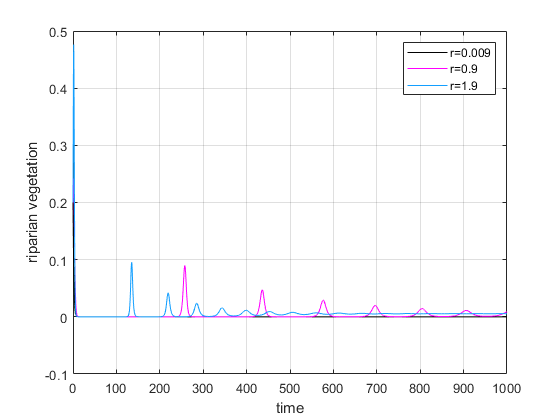
\includegraphics[width=\textwidth]{time_vs_riparian_r.png}
		\caption{Change in Riparian Vegetation with time} \label{fig:time_vs_riparian_r}
	\end{subfigure}
\hspace{0.08\textwidth}
        \begin{subfigure}[t]{0.45\textwidth}
                 \centering
         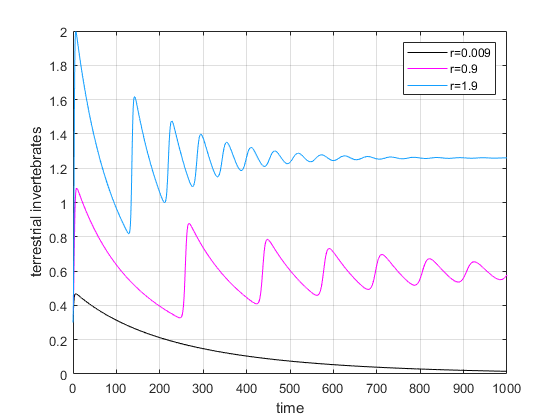
\includegraphics[width=\textwidth]{time_vs_invertebrates_r.png}
		\caption{Change in Terrestrial Invertebrates with time} \label{fig:time_vs_invertebrates_r}
	\end{subfigure}
\vskip\baselineskip
\begin{subfigure}[t]{0.45\textwidth}
                 \centering
         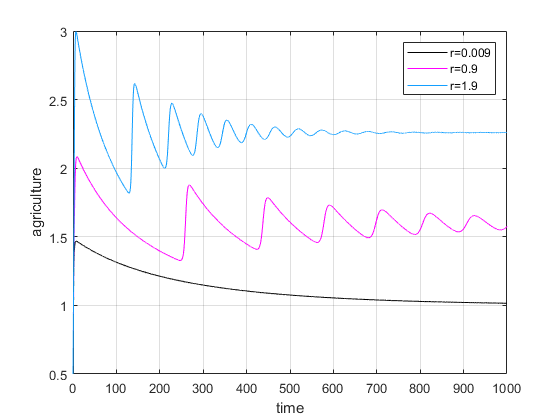
\includegraphics[width=\textwidth]{time_vs_agriculture_r.png}
		\caption{Change in Terrestrial Invertebrates with time} \label{fig:time_vs_agriculture_r}
	\end{subfigure}
\quad
              \begin{subfigure}[t]{0.45\textwidth}
                 \centering
         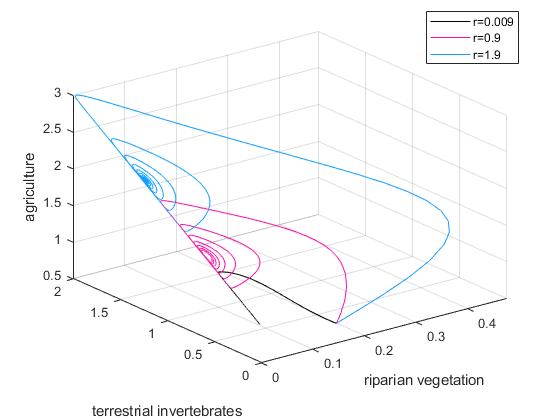
\includegraphics[width=\textwidth]{rip_inv_agr_r.png}
		\caption{Three dimensional change} \label{fig:rip_inv_agr_r}
	\end{subfigure}
\hspace{0.08\textwidth}
\end{figure}
\FloatBarrier
\begin{figure}[bp!]
	\centering
        \caption{Variation in parameter $\alpha$}
	\begin{subfigure}[t]{0.45\textwidth}
		\centering
	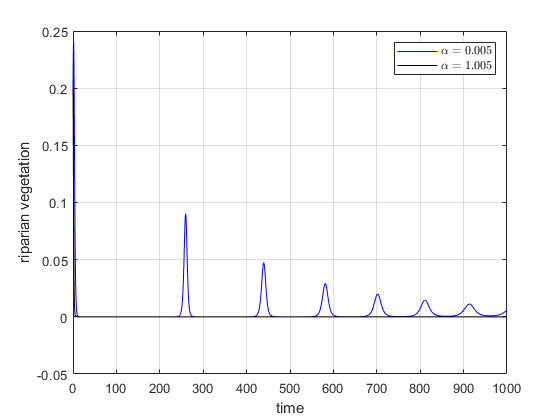
\includegraphics[width=\textwidth]{time_vs_riparian_alpha.png}
		\caption{Change in Riparian Vegetation with time} \label{fig:time_vs_riparian_alpha}
	\end{subfigure}
\hspace{0.08\textwidth}
        \begin{subfigure}[t]{0.45\textwidth}
                 \centering
         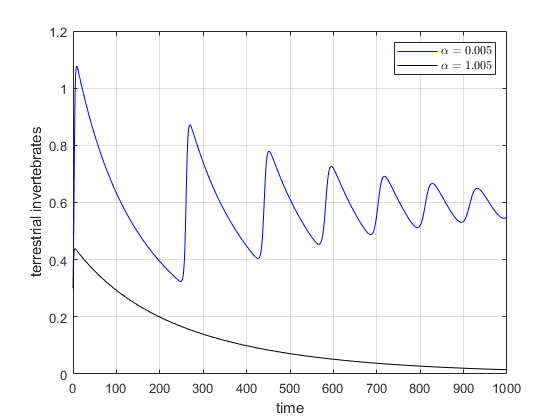
\includegraphics[width=\textwidth]{time_vs_invertebrates_alpha.png}
		\caption{Change in Terrestrial Invertebrates with time} \label{fig:time_vs_invertebrates_alpha}
	\end{subfigure}
\vskip\baselineskip
\begin{subfigure}[t]{0.45\textwidth}
                 \centering
         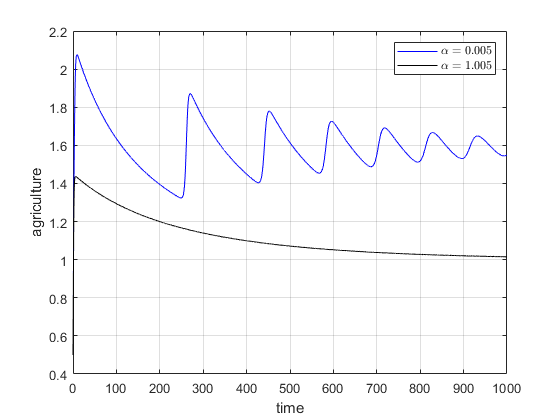
\includegraphics[width=\textwidth]{time_vs_agriculture_alpha.png}
		\caption{Change in Terrestrial Invertebrates with time} \label{fig:time_vs_agriculture_alpha}
	\end{subfigure}
\quad
              \begin{subfigure}[t]{0.45\textwidth}
                 \centering
         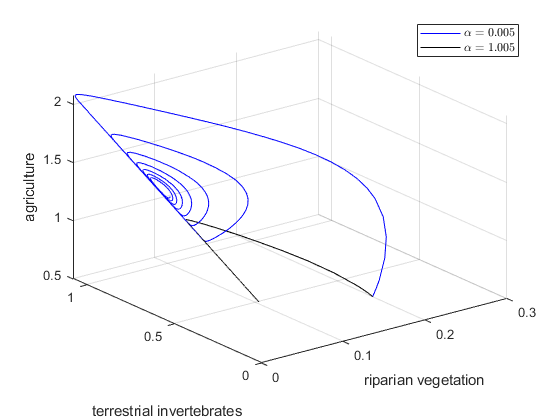
\includegraphics[width=\textwidth]{rip_inv_agr_alpha.png}
		\caption{Three dimensional change} \label{fig:rip_inv_agr_alpha}
	\end{subfigure}
\hspace{0.08\textwidth}
\end{figure}
\FloatBarrier
\begin{figure}[bp!]
	\centering
        \caption{Variation in parameter $\beta$}
	\begin{subfigure}[t]{0.45\textwidth}
		\centering
	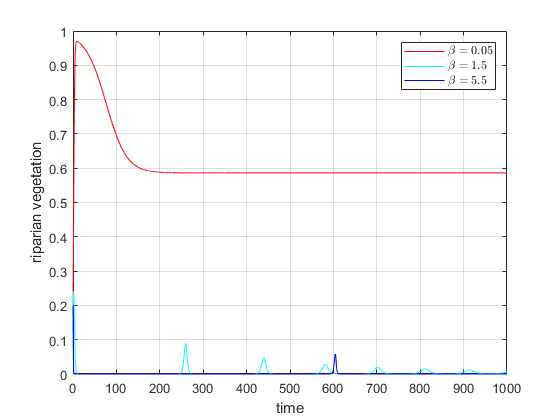
\includegraphics[width=\textwidth]{time_vs_riparian_beta.png}
		\caption{Change in Riparian Vegetation with time} \label{fig:time_vs_riparian_beta}
	\end{subfigure}
\hspace{0.08\textwidth}
        \begin{subfigure}[t]{0.45\textwidth}
                 \centering
         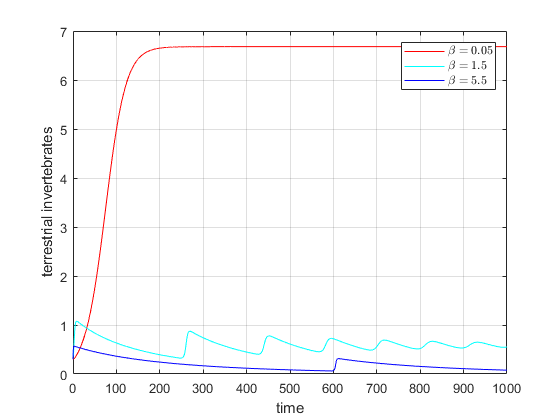
\includegraphics[width=\textwidth]{time_vs_invertebrates_beta.png}
		\caption{Change in Terrestrial Invertebrates with time} \label{fig:time_vs_invertebrates_beta}
	\end{subfigure}
\vskip\baselineskip
\begin{subfigure}[t]{0.45\textwidth}
                 \centering
         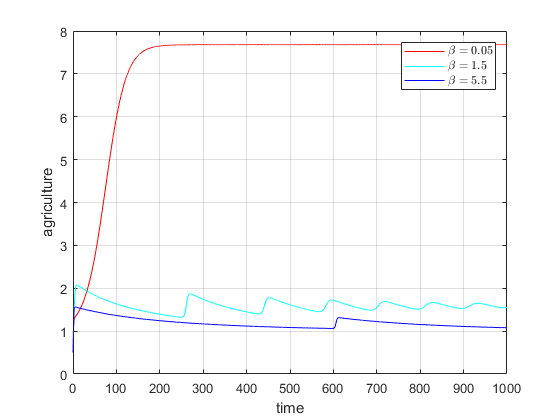
\includegraphics[width=\textwidth]{time_vs_agriculture_beta.png}
		\caption{Change in Terrestrial Invertebrates with time} \label{fig:time_vs_agriculture_beta}
	\end{subfigure}
\quad
              \begin{subfigure}[t]{0.45\textwidth}
                 \centering
         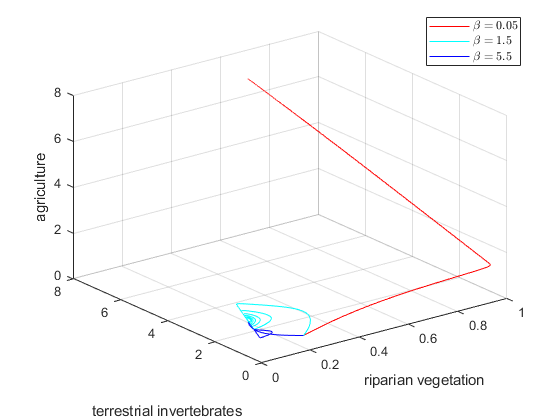
\includegraphics[width=\textwidth]{rip_inv_agr_beta.png}
		\caption{Three dimensional change} \label{fig:rip_inv_agr_beta}
	\end{subfigure}
\hspace{0.08\textwidth}
\end{figure}
\FloatBarrier
\begin{figure}[bp!]
	\centering
        \caption{Variation in parameter $\gamma$}
	\begin{subfigure}[t]{0.45\textwidth}
		\centering
	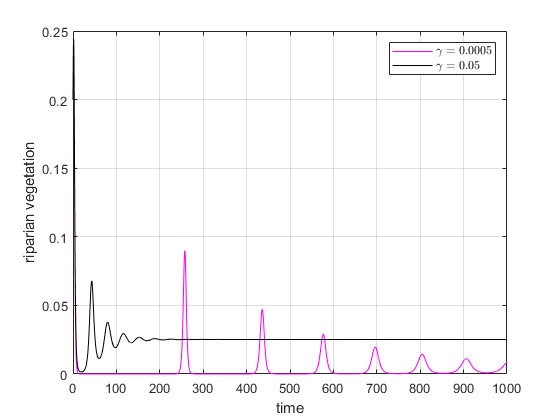
\includegraphics[width=\textwidth]{time_vs_riparian_gamma.png}
		\caption{Change in Riparian Vegetation with time} \label{fig:time_vs_riparian_gamma}
	\end{subfigure}
\hspace{0.08\textwidth}
        \begin{subfigure}[t]{0.45\textwidth}
                 \centering
         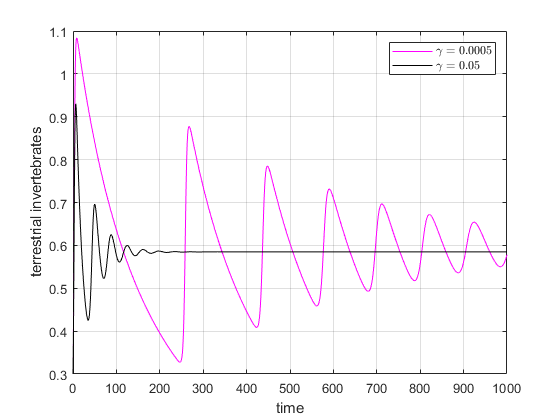
\includegraphics[width=\textwidth]{time_vs_invertebrates_gamma.png}
		\caption{Change in Terrestrial Invertebrates with time} \label{fig:time_vs_invertebrates_gamma}
	\end{subfigure}
\vskip\baselineskip
\begin{subfigure}[t]{0.45\textwidth}
                 \centering
         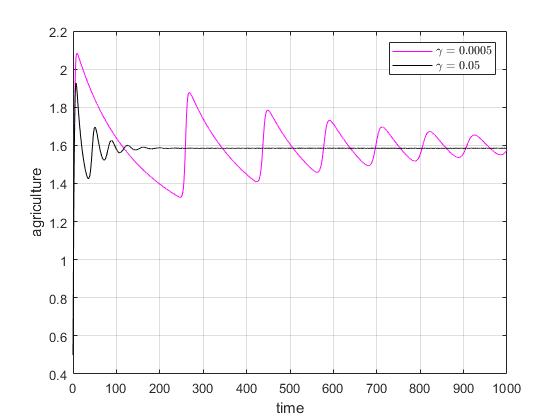
\includegraphics[width=\textwidth]{time_vs_agriculture_gamma.png}
		\caption{Change in Terrestrial Invertebrates with time} \label{fig:time_vs_agriculture_gamma}
	\end{subfigure}
\quad
              \begin{subfigure}[t]{0.45\textwidth}
                 \centering
         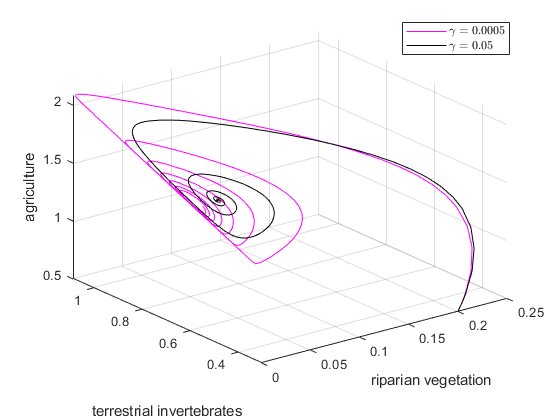
\includegraphics[width=\textwidth]{rip_inv_agr_gamma.png}
		\caption{Three dimensional change} \label{fig:rip_inv_agr_gamma}
	\end{subfigure}
\hspace{0.08\textwidth}
\end{figure}
\FloatBarrier
\begin{figure}[bp!]
	\centering
        \caption{Variation in parameter $\delta$}
	\begin{subfigure}[t]{0.45\textwidth}
		\centering
	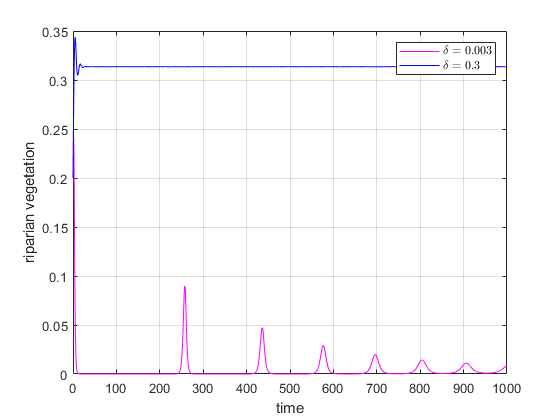
\includegraphics[width=\textwidth]{time_vs_riparian_delta.png}
		\caption{Change in Riparian Vegetation with time} \label{fig:time_vs_riparian_delta}
	\end{subfigure}
\hspace{0.08\textwidth}
        \begin{subfigure}[t]{0.45\textwidth}
                 \centering
         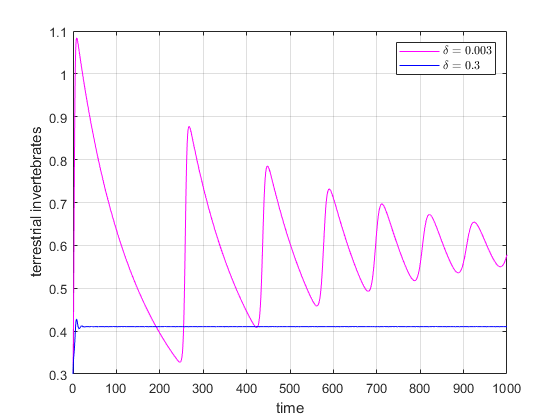
\includegraphics[width=\textwidth]{time_vs_invertebrates_delta.png}
		\caption{Change in Terrestrial Invertebrates with time} \label{fig:time_vs_invertebrates_delta}
	\end{subfigure}
\vskip\baselineskip
\begin{subfigure}[t]{0.45\textwidth}
                 \centering
         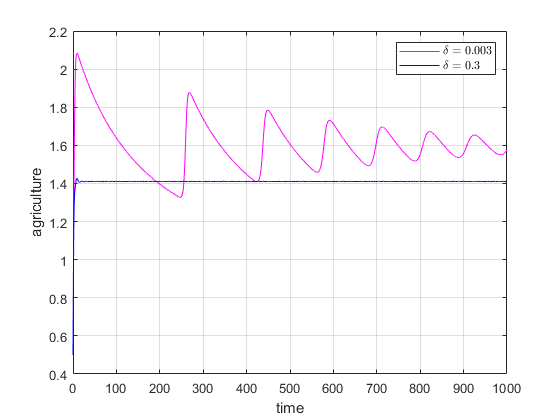
\includegraphics[width=\textwidth]{time_vs_agriculture_delta.png}
		\caption{Change in Terrestrial Invertebrates with time} \label{fig:time_vs_agriculture_delta}
	\end{subfigure}
\quad
              \begin{subfigure}[t]{0.45\textwidth}
                 \centering
         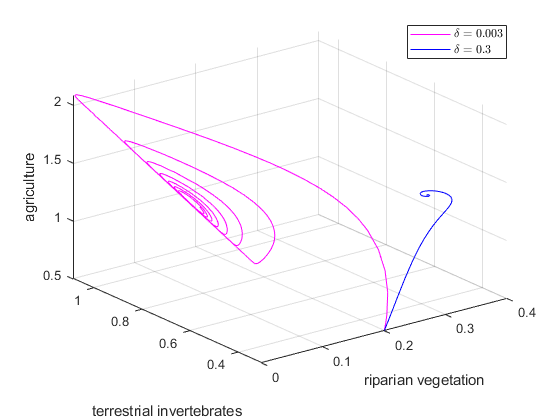
\includegraphics[width=\textwidth]{rip_inv_agr_delta.png}
		\caption{Three dimensional change} \label{fig:rip_inv_agr_delta}
	\end{subfigure}
\hspace{0.08\textwidth}
\end{figure}
%%%REFERENCES
\begin{thebibliography}{99}
\bibitem{pettit2007fire}
  Pettit, N. E., \& Naiman, R. J. (2007). Fire in the riparian zone: characteristics and ecological consequences. Ecosystems, 10(5), 673-687.
\bibitem{popescu2021riparian}
  Popescu, C., Oprina-Pavelescu, M., Dinu, V., Cazacu, C., Burdon, F. J., Forio, M. A. E., ... \& Rîșnoveanu, G. (2021). Riparian vegetation structure influences terrestrial invertebrate communities in an agricultural landscape. Water, 13(2), 188.
\bibitem{hood2000}
  Hood, W. G., \& Naiman, R. J. (2000). Vulnerability of riparian zones to invasion by exotic vascular plants. Plant ecology, 148(1), 105-114.
\bibitem{richardson2007}
  Richardson, D. M., Holmes, P. M., Esler, K. J., Galatowitsch, S. M., Stromberg, J. C., Kirkman, S. P., ... \& Hobbs, R. J. (2007). Riparian vegetation: degradation, alien plant invasions, and restoration prospects. Diversity and distributions, 13(1), 126-139.
\bibitem{burdon2020assessing}
  Burdon, F. J., Ramberg, E., Sargac, J., Forio, M. A. E., De Saeyer, N., Mutinova, P. T., ... \& McKie, B. G. (2020). Assessing the benefits of forested riparian zones: A qualitative index of riparian integrity is positively associated with ecological status in European streams. Water, 12(4), 1178.
\bibitem{cesarini2022riparian}
  Cesarini, G., \& Scalici, M. (2022). Riparian vegetation as a trap for plastic litter. Environmental Pollution, 292, 118410.
\bibitem{alemu2018identifying}
  Alemu, T., Weyuma, T., Alemayehu, E., \& Ambelu, A. (2018). Identifying riparian vegetation as indicator of stream water quality in the Gilgel Gibe catchment, southwestern Ethiopia. Ecohydrology, 11(1), e1915.
\bibitem{ssymank2008pollinating}
  Ssymank, A., Kearns, C. A., Pape, T., \& Thompson, F. C. (2008). Pollinating flies (Diptera): a major contribution to plant diversity and agricultural production. Biodiversity, 9(1-2), 86-89.
\bibitem{forio2020small}
  Forio, M. A. E., De Troyer, N., Lock, K., Witing, F., Baert, L., Saeyer, N. D., ... \& Goethals, P. (2020). Small patches of riparian woody vegetation enhance biodiversity of invertebrates. Water, 12(11), 3070.
\bibitem{andersen2000long}
  Andersen, A., \& Eltun, R. (2000). Long‐term developments in the carabid and staphylinid (Col., CArabidae and Staphylinidae) fauna during conversion from conventional to bilogivcal farming. Journal of Applied Entomology, 124(1), 51-56.
\bibitem{burdon2013habitat}
  Burdon, F. J., McIntosh, A. R., \& Harding, J. S. (2013). Habitat loss drives threshold response of benthic invertebrate communities to deposited sediment in agricultural streams. Ecological Applications, 23(5), 1036-1047.
\bibitem{steward2022}
  Steward, A. L., Datry, T., \& Langhans, S. D. (2022). The terrestrial and semi‐aquatic invertebrates of intermittent rivers and ephemeral streams. Biological Reviews.
\bibitem{heartsill2003riparian}
  Heartsill-Scalley, T., \& Aide, T. M. (2003). Riparian vegetation and stream condition in a tropical agriculture–secondary forest mosaic. Ecological Applications, 13(1), 225-234.
\bibitem{corbacho2003patterns}
  Corbacho, C., Sánchez, J. M., \& Costillo, E. (2003). Patterns of structural complexity and human disturbance of riparian vegetation in agricultural landscapes of a Mediterranean area. Agriculture, Ecosystems \& Environment, 95(2-3), 495-507.
\bibitem{schlosser1981riparian}
  Schlosser, I. J., \& Karr, J. R. (1981). Riparian vegetation and channel morphology impact on spatial patterns of water quality in agricultural watersheds. Environmental Management, 5(3), 233-243.
\bibitem{flory1999}
Flory, E. A., \& Milner, A. M. (1999). Influence of riparian vegetation on invertebrate assemblages in a recently formed stream in Glacier Bay National Park, Alaska. Journal of the North American Benthological Society, 18(2), 261-273.
\bibitem{kawaguchi2001}
  Kawaguchi, Y., \& Nakano, S. (2001). Contribution of terrestrial invertebrates to the annual resource budget for salmonids in forest and grassland reaches of a headwater stream. Freshwater Biology, 46(3), 303-316.
\bibitem{wipfli1997}
  Wipfli, M. S. (1997). Terrestrial invertebrates as salmonid prey and nitrogen sources in streams: contrasting old-growth and young-growth riparian forests in southeastern Alaska, USA. canadian Journal of Fisheries and aquatic sciences, 54(6), 1259-1269.
\bibitem{sabo2002}
  Sabo, J. L., Bastow, J. L., \& Power, M. E. (2002). Length–mass relationships for adult aquatic and terrestrial invertebrates in a California watershed. Journal of the North American Benthological Society, 21(2), 336-343.
\bibitem{you2015}
  You, X., Liu, J., \& Zhang, L. (2015). Ecological modeling of riparian vegetation under disturbances: a review. Ecological modelling, 318, 293-300.
\bibitem{burdon2020}
  Burdon, F. J. (2020). Agriculture and mining contamination contribute to a productivity gradient driving cross-ecosystem associations between stream insects and riparian arachnids. In Contaminants and Ecological Subsidies (pp. 61-90). Springer, Cham.
\bibitem{edwards1996effect}
  Edwards, E. D., \& Huryn, A. D. (1996). Effect of riparian land use on contributions of terrestrial invertebrates to streams. Hydrobiologia, 337(1), 151-159.
\bibitem{ramey2017terrestrial}
  Ramey, T. L., \& Richardson, J. S. (2017). Terrestrial invertebrates in the riparian zone: mechanisms underlying their unique diversity. BioScience, 67(9), 808-819.
\bibitem{ruetz2003interspecific}
  Ruetz III, C. R., Hurford, A. L., \& Vondracek, B. (2003). Interspecific interactions between brown trout and slimy sculpin in stream enclosures. Transactions of the American Fisheries Society, 132(3), 611-618.
\bibitem{krell2015aquatic}
  Krell, B., Röder, N., Link, M., Gergs, R., Entling, M. H., \& Schäfer, R. B. (2015). Aquatic prey subsidies to riparian spiders in a stream with different land use types. Limnologica, 51, 1-7.
\bibitem{riis2020global}
  Riis, T., Kelly-Quinn, M., Aguiar, F. C., Manolaki, P., Bruno, D., Bejarano, M. D., ... \& Dufour, S. (2020). Global overview of ecosystem services provided by riparian vegetation. BioScience, 70(6), 501-514.
\bibitem{stockan2014effects}
  Stockan, J. A., Baird, J., Langan, S. J., Young, M. R., \& Iason, G. R. (2014). Effects of riparian buffer strips on ground beetles (Coleoptera, Carabidae) within an agricultural landscape. Insect Conservation and Diversity, 7(2), 172-184.
\bibitem{cole2012riparian}
  Cole, L. J., Brocklehurst, S., Elston, D. A., \& McCracken, D. I. (2012). Riparian field margins: can they enhance the functional structure of ground beetle (Coleoptera: Carabidae) assemblages in intensively managed grassland landscapes?. Journal of Applied Ecology, 49(6), 1384-1395.
\bibitem{greenwood1995patial}
  Greenwood, M. T., Bickerton, M. A., \& Petts, G. E. (1995). Patial distribution of spiders on the floodplain of the river trent, UK: The role of hydrological setting. Regulated Rivers: Research \& Management, 10(2‐4), 303-313.
\bibitem{gakkhar2012control}
  Gakkhar, S., \& Singh, A. (2012). Control of chaos due to additional predator in the Hastings–Powell food chain model. Journal of Mathematical Analysis and Applications, 385(1), 423-438.
\bibitem{nagumo1942}
  Nagumo, M. (1942). ber die lage der integralkurven gewhnlicher differentialgleichungen. Proceedings of the Physico-Mathematical Society of Japan. 3rd Series, 24, 551-559.
\bibitem{hale1969}
  Hale JK (1969) Ordinary differential equations. Wiley-Interscience, New York.
\bibitem{freedman1985}
  Freedman, H. I., \& So, J. H. (1985). Global stability and persistence of simple food chains. Mathematical biosciences, 76(1), 69-86.
\end{thebibliography}
%% TABLE FOR PARAMETER DEFINITION
\begin{table}[htp!] \label{Table 1}
	\renewcommand{\arraystretch}{2}
	\caption{\textbf{: Description of Model Parameters}}
	\begin{center}
		\begin{tabular}{|p{2cm}||p{9cm}||p{5cm}|}
        \hline
			% after \\: \hline or \cline{col1-col2} \cline{col3-col4} ...
			\textbf{Parameter} & \textbf{Definition} \\
			\hline
			$r$ & Instrinsic growth rate of vegetation\\
			\hline
			${K}$ & Carrying capacity of vegetation\\
			\hline
			${\alpha}$ & Depletion of vegetation due to enroachment for agricultural production\\
			\hline
			${\beta}$ & Depletion rate of vegetation due to its use by invertebrates\\
			\hline
			${\theta}$ & Proportion of $\beta$ that is used by invertebrates for its growth\\
		    \hline
			${\gamma}$ & Intra-specific competition rate of invertebrates\\
		    \hline
			${\delta}$ & Depletion rate of invertebrates due to agriculture\\
		    \hline
			${s}$ & Intrinsic growth rate of agricultural production\\
			\hline
			${L}$ & Carrying capacity of agricultural production\\
			\hline
			${\nu}$ & Growth of agriculture due to invertebrate\\
			\hline			
		\end{tabular}\label{Table 1}
	\end{center}
\end{table}
%%%% TABLE FOR COEXISTENCES
\begin{landscape}
  \begin{table}[htp!]\label{Table 2}
\caption{\textbf{: Coexistence equilibrium and its existence conditions}}
\begin{center}
\begin{tabular}{|L||L||L||c||c|}
\hline
			
			\textbf{Discriminant} & \textbf{Values of $\tilde a$} & \textbf{Values of $\tilde b, \tilde c$} & \textbf{Values of $\tilde V$} & \textbf{Feasible Coexistence equilibrium} \\
\hline
\hline
$\Delta_{E_3}<0$ & -----------& ----------- & Complex $\tilde V_1$ \& $\tilde V_2$ & ----\\ \hline
\hline
\multirow{1}{*}{$\Delta_{E_3}=0$} & \multicolumn{1}{|c|}{$\tilde a>0$} & \multicolumn{1}{|c|}{$\tilde b>0,\tilde c<0$} & \multirow{1}{*}{Positive coincident $\tilde V_1$ \& $\tilde V_2$}  & \multirow{1}{*}{Coincident $E_{3^*}$ exists}\\\hline
                                \hline
\multirow{3}{*}{$\Delta_{E_3}>0$} & \multirow{3}{*}{$\tilde a>0$} & \multicolumn{1}{|c|}{$\tilde b>0,\tilde c<0$} & \multicolumn{1}{|c|}{$\tilde V_1$ is positive \& $\tilde V_2$ is negative} & \multicolumn{1}{|c|}{Either one or both of $E_{3_1}$ \& $E_{3_2}$ may exist}\\\cline{3-5}
                                  &                          & \multicolumn{1}{|c|}{$\tilde b=0,\tilde c<0$} & \multicolumn{1}{|c||}{$\tilde V_1$ is positive \& $\tilde V_2$ is negative} & \multicolumn{1}{|c|}{---}\\\cline{3-5}
                                  &                          & \multicolumn{1}{|c||}{$\tilde b<0,\tilde c<0$} & \multicolumn{1}{|c||}{$\tilde V_1$ is positive \& $\tilde V_2$ is negative} & \multicolumn{1}{|c|}{---}\\\hline
         \end{tabular}\label{Table 2}
         \end{center}
         \end{table}
\end{landscape}
\end{document}
